\section{ESN Results}
\label{sec:esn-results}

In this section we show the prediction skill of the more generic ESN
architecture outlined in \cref{subsec:rc}.
Here we use similar metrics as in \cref{sec:nvar-results} to evaluate the ESN
skill, except that we show time averaged quantitative metrics because all of the
ESN predictions are stable for the full 12~hour forecast horizon.

\subsection{Global Parameter Optimization}
\label{subsec:esn-ego}

% Here we present ESN results, using mainly the two metrics used to evaluate
% NVAR
In this section we show the prediction skill of the more generic ESN
architecture outlined in \red{SUBSEC}.
As noted in the ESN literature, prediction skill is highly dependent on the
scalar hyperparameters \red{REF}.
Because optimal parameter values can vary widely for different dynamical
systems, we use a Bayesian Optimization algorithm to find values that perform
well.
Here, we use the following objective function
\begin{linenomath*}\begin{equation}
    \cf_\text{macro}(\hyperparameters_{RC}) =
    \text{NRMSE} + \gamma \text{KE\_NRMSE}
\end{equation}\end{linenomath*}
where $\gamma$ controls the degree to which we penalize deviations from the 1D
Kinetic Energy Density spectrum.
Our motivation to use this penalty term in the objective function stems from the
results by \red{Platt et al ??} who show that adding invariant properties to the
macro cost function in this way improves the optimizer's ability to
select optimal parameters.
Because our goal is to understand how well these ML models can forecast
all scales of turbulent motions, we use the KE spectrum.

\cref{fig:esn-error-vs-gamma} shows how the additional term in the cost function influences
prediction skill, using an ESN with $\nsub=1$, i.e., at the model timestep.
There is a clear tradeoff between NRMSE and KE error: as $\gamma$ increases the
NRMSE decreases but the spectral representation improves.
\cref{fig:esn-ke-error-vs-gamma} shows the KE Density relative error as a function of $\gamma$
(color), indicating how this tradeoff manifests.
When $\gamma=0$, the ESN global parameters are chosen to minimize NRMSE, leading
to blurry predictions and a dampened spectrum at the higher wavenumbers,
especially for $|\mathbf{K}| > 2\cdot10^{-3}$~rad~km$^{-1}$.
On the other hand, when $\gamma = 0.1$, the global parameters are chosen to
minimize both NRMSE and KE density error.
In this case, KE relative error is reduced by more than a factor of two and the
dampening of the energy spectrum is much more muted.
However, NRMSE increases by roughly 20\% and KE relative error increases at
larger spatial scales,
$|\mathbf{K} \lessapprox 10^{-3}$~rad~km$^{-1}$.
Note that the KE error can be small at the large scales but still throw off the
NRMSE.

\begin{figure}
    \centering
    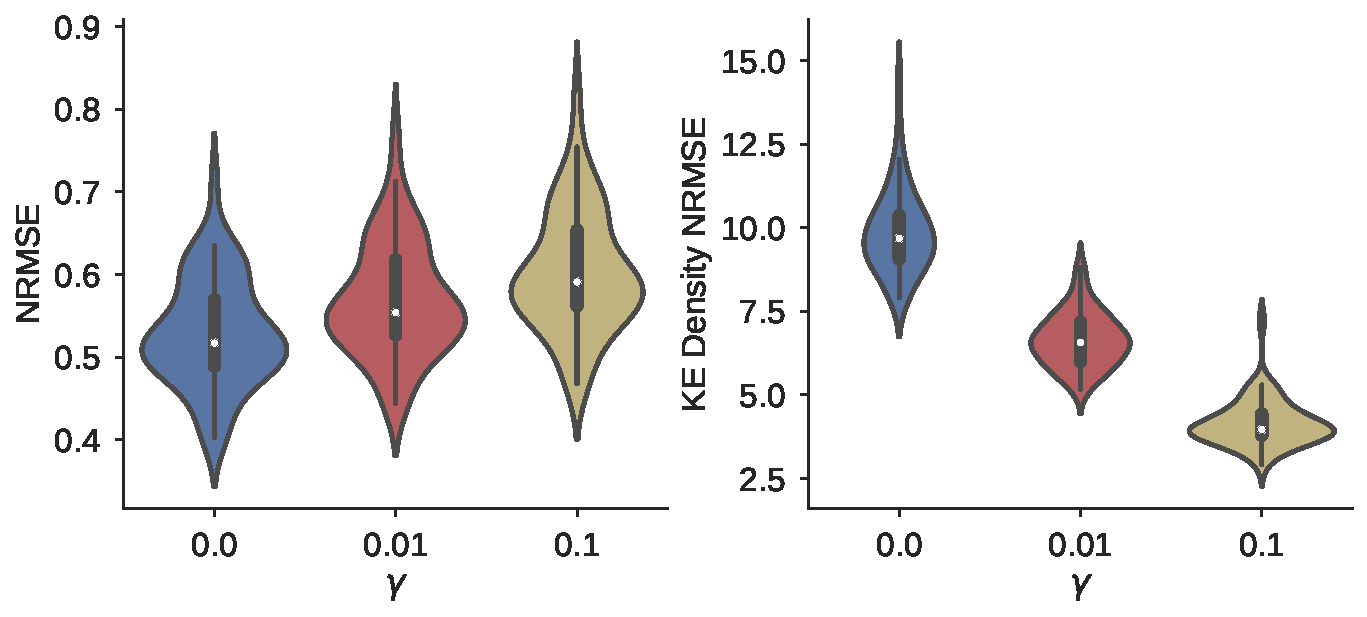
\includegraphics[width=.8\textwidth]{../figures/rc_nrmse_and_kenrmse_nsub01.pdf}
    \caption{$\nsub=1$ error tradeoff}
    \label{fig:esn-error-vs-gamma}
\end{figure}

\begin{figure}
    \centering
    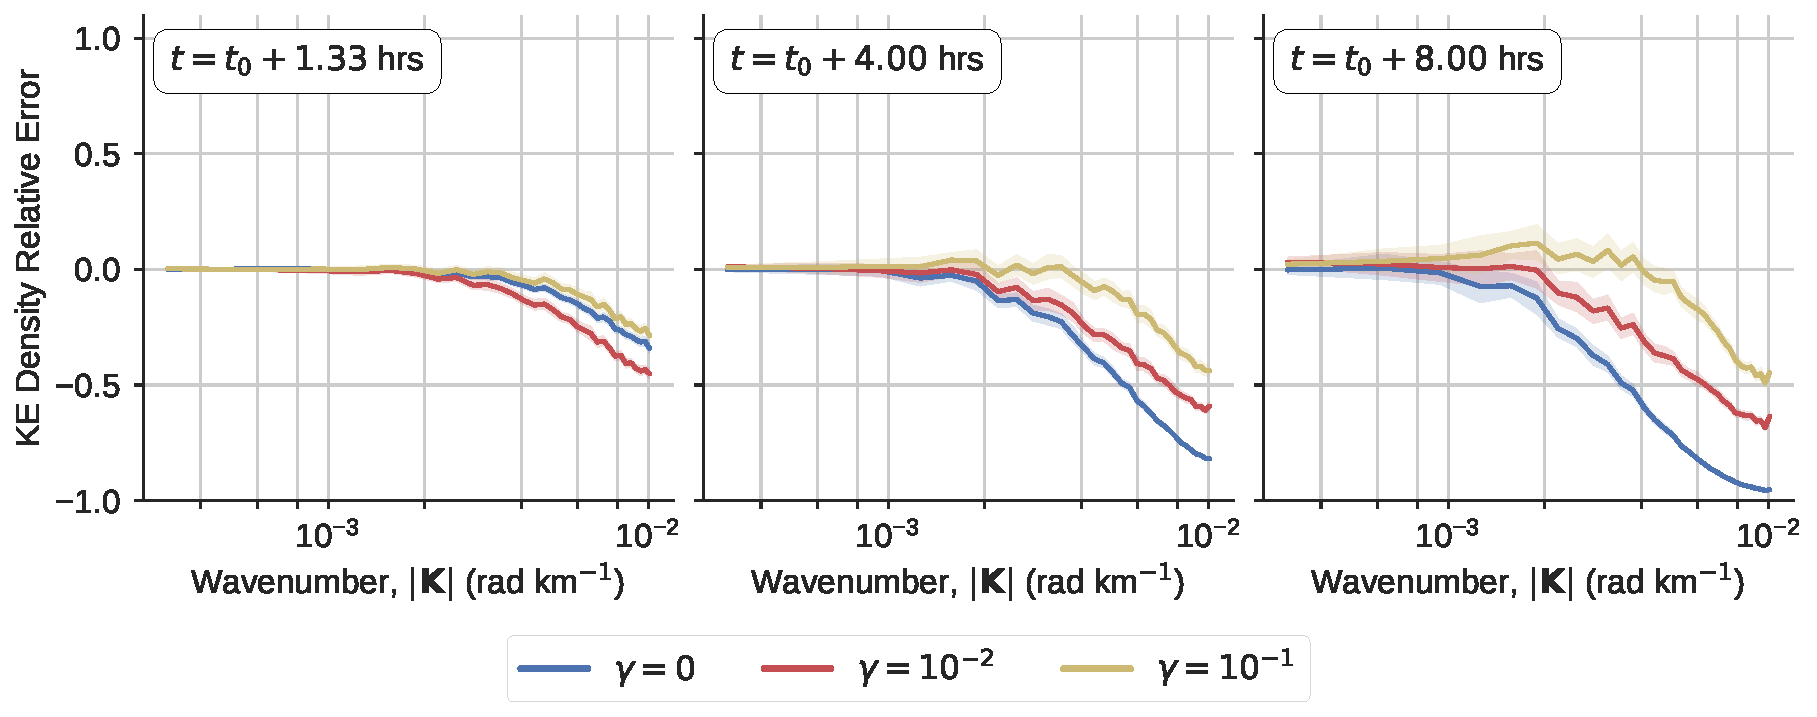
\includegraphics[width=.8\textwidth]{../figures/rc_ke_rel_err_nsub01.pdf}
    \caption{$\nsub=1$ scales of the error tradeoff}
    \label{fig:esn-ke-error-vs-gamma}
\end{figure}

We surmise that the tradeoff between NRMSE and KE NRMSE is therefore really
indicative of an ability to represent the small and large scales of motion.
Features that are characteristic of wavenumbers $> 10^{-3}$ are likely to have
little influence on NRMSE, while the larger features dominate.
Because the KE NRMSE treats all scales equally, this gives us the best chance to
find a model that captures all scales of motion well.
Unfortunately it appears that by additionally incorporating the KE spectrum,
there one cannot obtain both the large and small scales: one must choose.



\subsection{The effect of temporal subsampling}
\label{subsec:esn-subsampling}


The NVAR predictions shown in \cref{subsec:nvar-subsampling} indicated that
subsampling the training data increases spectral bias.
However, the architecture was not designed to have a good spectral
representation.
The previous section showed that by optimizing the global ESN parameters, the
spectral bias can be reduced.
Here, we explore the following question: does temporal subsampling still
increase spectral bias in the more general ESN framework, even when parameters
are chosen to minimize this bias?

\cref{fig:esn-best-spec-error-vs-nsub} shows the NRMSE and KE Density NRMSE as a
function of the temporal subsampling factor $\nsub$.
In each of these cases we set $\gamma=0.1$, and we note that larger values
produced similar results.
The right panel shows that KE Density NRMSE increases with $\nsub$, indicating
that temporal subsampling does lead to some inherent degree of spectral bias.
We note that the overall shape of the KE Density Relative Error is similar for
each (i.e., similar to the yellow curve in \cref{fig:esn-ke-error-vs-gamma}),
but error is simply larger in amplitude as $\nsub$ grows.

\begin{figure}
    \centering
    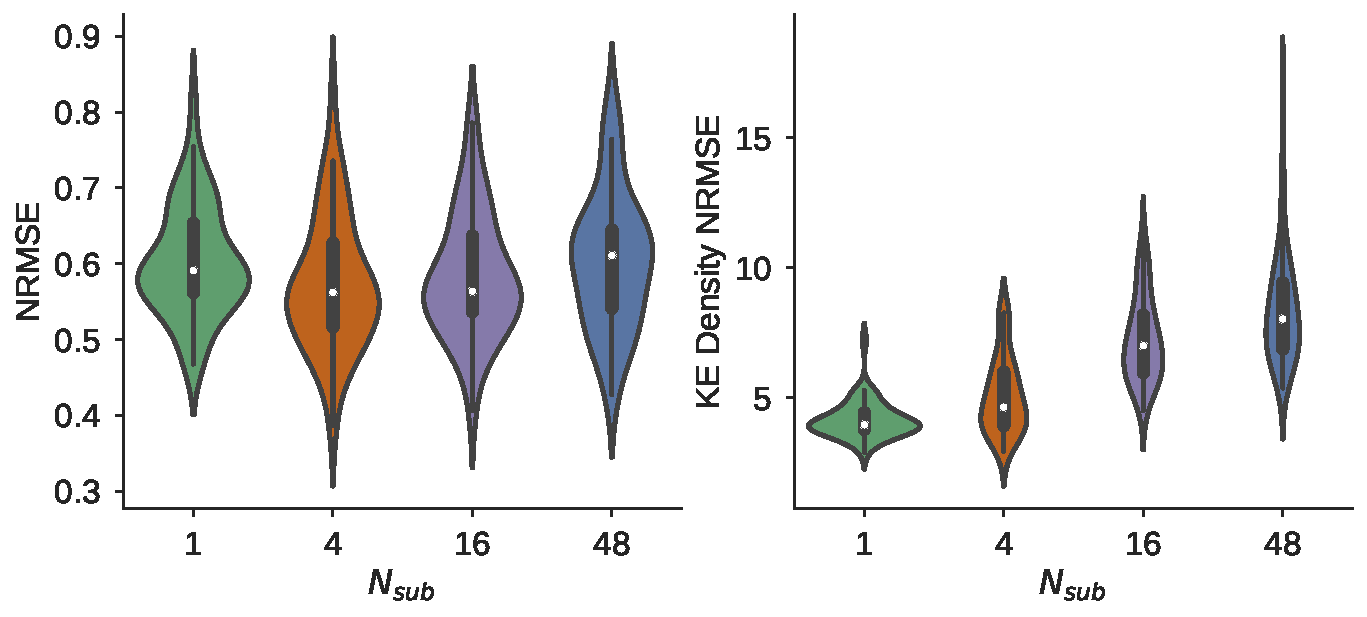
\includegraphics[width=.8\textwidth]{../figures/rc_nrmse_kenrmse_gamma0.1.pdf}
    \caption{Best spectral error, $\gamma=0.1$}
    \label{fig:esn-best-spec-error-vs-nsub}
\end{figure}

Interestingly, the NRMSE between each $\nsub$ case is essentially the same, and
is not even lowest at the model timestep ($\nsub=1$).
Therefore, if the goal is to simply produce a prediction with minimal RMSE over a
12~hour window, then at least some degree is beneficial due to improvements in
computational efficiency.
Moreover, \cref{fig:esn-best-nrmse-vs-nsub} shows that this is also true
even when $\gamma=0$, i.e., when NRMSE is the only criterion for parameter
choice.
In this case, there is no strong trend in the KE Density NRMSE.
We suggest that this result indicates that NRMSE alone is not the best criteria
for model selection, especially when the representation of spatial features or
spectral properties is desired.

\begin{figure}
    \centering
    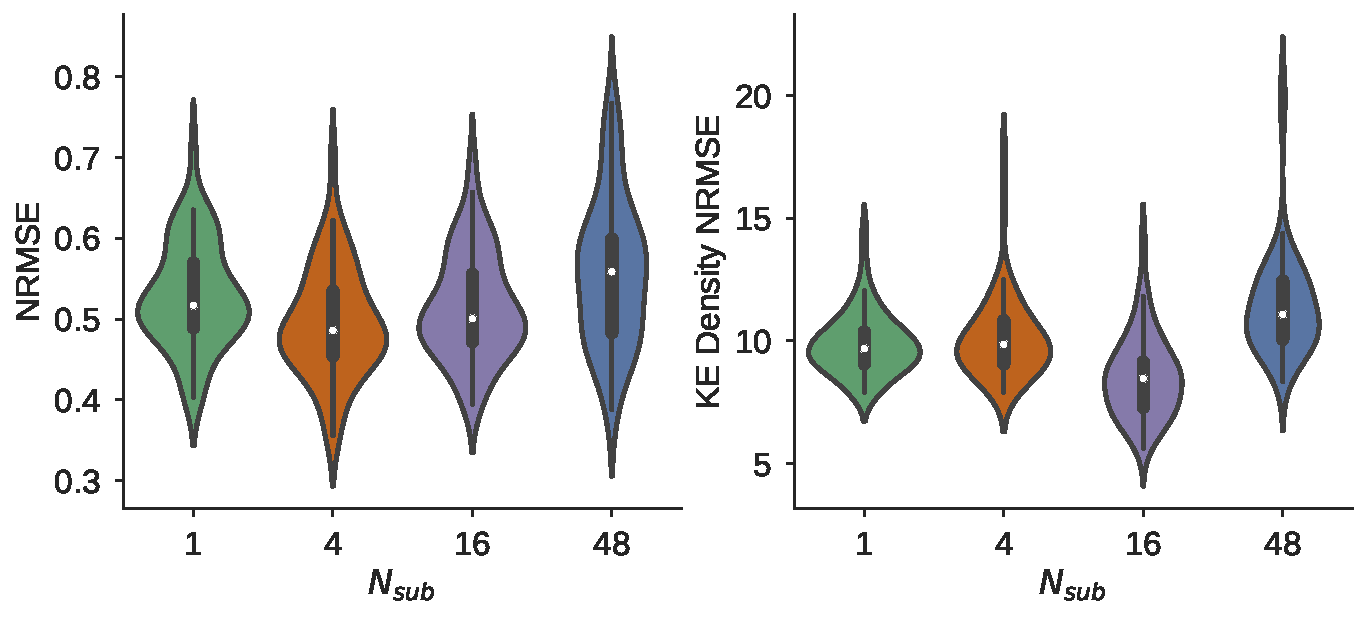
\includegraphics[width=.8\textwidth]{../figures/rc_nrmse_kenrmse_gamma0.0.pdf}
    \caption{Best NRMSE, $\gamma=0$}
    \label{fig:esn-best-nrmse-vs-nsub}
\end{figure}


\subsection{Transferability of global parameters}

Are the optimal parameters that we obtain from highly subsampled runs
transferabble to the Nsub=1?
In order to make training more efficient.

\subsection{Impact of reservoir size, overlap}

Maybe supplement

